% !TeX encoding = UTF-8

\documentclass{LTHtwocol} % Use this when you work on your report.
% \documentclass[final]{LTHtwocol} % Use this for the final version.
                                   % It will remove page numbers and
                                   % markers for overfull boxes.
                                   % There really shouldn't be any of those anyway.

\usepackage[utf8]{inputenc}
\usepackage{amsmath,amssymb,graphicx}
\usepackage{float}
\usepackage[table,xcdraw]{xcolor}
\usepackage{hyperref}
\usepackage{algorithm}
\usepackage{algpseudocode}
\hypersetup{
	colorlinks,
	linkcolor={red!50!black},
	citecolor={blue!50!black},
	urlcolor={blue!80!black}
}

\usepackage{kantlipsum} % Only for the dummy text. Remove for your own report.

\addbibresource{bibliography.bib}

% Custom commands
% From: https://tex.stackexchange.com/questions/130307/questions-about-algpseudocode
\algnewcommand\True{\textbf{true}\space}
\algnewcommand\False{\textbf{false}\space}

% Document begins here
\begin{document}
\begin{frontmatter}
\title{Balancing a Double Inverted Pendulum on Cart} % Title of the project.
                      							 % Note that all reports are in English,
							                     %so that our international students can read them.

\author[cem]{Cem Alpt\"urk}
\author[pukashawar]{Pukashawar Pannu}

\email[cem]{ce5368al-s@student.lu.se}
\email[pukashawar]{pu6218pa-s@student.lu.se}

\begin{abstract}
    Controlling a double inverted pendulum on a cart is an inherently difficult problem.
    The system is chaotic meaning that the dynamics cannot be predicted over a longer time span.
    A way to control such a system is to use the current state to determine an action that moves the cart appropriately to balance the double pendulum.
    One such way is by reinforcement learning.
    The approach in this project uses a model free controller trained with Deep Q-learning to control the double pendulum.
    Benefits of Deep Q-learning over regular Q-learning is that the controller can be used for situations that are not presented during training.
    This has been confirmed in the results for the single pendulum model, an easier problem to control that was used to confirm the implementation of the learning algorithm.
    Results for the double pendulum controller are pending.
    % The abstract should be a 200--250 word compact description of your project. What was the objective? Which methods did you use? What was the (main) result?
\end{abstract}

\end{frontmatter}

% Stick to the proposed structure below. Add \subsections{} as appropriate.
% This file compiles on the Automatic Control Department system by typing the
% following into the terminal (while in the directory of the file, and with all
% other files belonging to the template untouched):
% > pdflatex template
% > biber template
% The first line compiles the .tex file. The second line generates the
% bibliography. Once this is done, you may need to run the first line 1-2
% additional times, for the system to get all cross references right in the
% produced pdf output.

\section{Introduction}
The goal of this project is to teach an agent to control a double pendulum on a cart to be standing upright, in its equilibrium point, using reinforcement learning.
A double pendulum is a highly chaotic system, where its behavior heavily depends on its initial conditions.
As a result, this system can be very difficult to control.
Figure \ref{fig:double_pendulum_chaotic} shows a simulation with 4 double pendulums with nearly identical initial conditions.
After some time their behaviors become so different that it becomes nearly impossible to make a prediction about the future.
This illustrates the chaotic behavior of this system.
Our aim is to create an agent that can learn from its own experiences to control the double pendulum, by applying a force on the cart in the horizontal direction, such that it stays upright.
Although this is an academic problem, the results could be applied to any type of learning problem since the agent is unaware of what it's working on.
\cite{qlearning_first}
\begin{figure}[H]
	\centering
	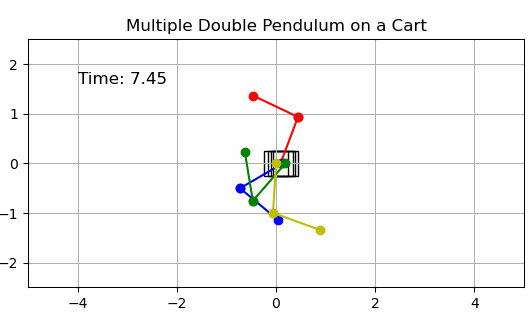
\includegraphics[width=0.9\columnwidth]{figures/Double_Pendulum_Chaotic.PNG}
	\label{fig:double_pendulum_chaotic}
	\caption{4 double pendulums simulated with similar initial conditions after $9.86$ seconds, with a difference of $0.02 rad/s$ differences on the inner pendulum angular velocities. All other initial states were equal.}
\end{figure}
% Here you introduce the project. What is the background? What project do you aim at solve? References to prior work? If the project makes a positive or negative environmental, or other solitary, impact, describe it here. Are there any ethical considerations? You might want to reference relevant literature, e.g. \cite{openclosed2, Hellerstein2004, Yun2015}. A general \LaTeX\ guide is available at \cite{latexwiki}.

\subsection{Reinforcement Learning}
%\kant[1] % This generates the dummy text
The main idea of reinforcement learning is to learn to make decisions based on past experiences.
In this case this means to train an agent that performs the best action, the force applied in the horizontal direction,  possible given the current states of the system.
For each action taken by the agent, the environment returns a new state and a reward for that action.
The reward is calculated based on how close the system is to its equilibrium point.
The goal of training the agent is to optimize gained reward for each action taken.

\section{Modeling}
The system consists of a cart that can move in the horizontal direction and two pendulums that are coupled to each other such that there is no collision between any parts.
Since this project is not about modeling the double pendulum, but rather about controlling it, we have borrowed the equations of motion from \cite{Double_Pendulum_Equations}.
The states of the system are represented by,
\begin{equation}
x  :=
\begin{bmatrix}
y & \dot{y}
\end{bmatrix}
^T , \quad y :=
\begin{bmatrix}
q & \theta_1 & \theta_2
\end{bmatrix}
^T
\end{equation}
%\begin{equation}
%x :=
%\begin{bmatrix}
%q & \theta_1 &  \theta_2 &  \dot{q} &  \dot{\theta_1} & \dot{\theta_2}
%\end{bmatrix}
% ^T
%\end{equation}
\begin{itemize}
\item $q$ is the position of the cart on the horizontal axis.
\item $\theta_1$ is the angle of the inner pendulum with respect to the vertical axis in the clockwise direction.
\item $\theta_2$ is the angle of the outer pendulum with respect to the vertical axis in the clockwise direction.
\item $\dot{q}$ is the velocity of the cart in the horizontal axis.
\item $\dot{\theta_1}$ is the angular velocity of the inner pendulum.
\item $\dot{\theta_2}$ is the angular velocity of the outer pendulum.
\end{itemize}

The system parameters are represented by,
\begin{itemize}
\item $m = 1 [kg]$ is the mass of the cart.
\item $m_1 = 0.1 [kg]$ is the mass of the inner pendulum.
\item $m_2 = 0.1[kg]$ is the mass of the outer pendulum.
\item $l_1 = 1 [m]$ is the length of the inner pendulum.
\item $l_2 = 1[m]$ is the length of the outer pendulum.
\item $g = 9.81 [m/s^2]$ is the gravitational acceleration.
 \end{itemize}

The equations of motions for this system \cite{Double_Pendulum_Equations}, are adjusted such there is no friction or disturbances.
The input to the system is a horizontal force that is acting on the cart, represented by $u$ $[N]$.

\begin{equation}
M(y) \ddot{y} = f(y,\dot{y},u)
\end{equation}


\begin{equation}
\resizebox{ \columnwidth}{!}
{
$
M(y) :=
\begin{bmatrix}
m + m_1 +m_2 & l_1(m_1+m_2)\cos \theta_1 & m_2 l_2 \cos \theta_2 \\
l_1 (m_1 + m_2) \cos \theta_1 & l_1^2(m_1+m_2) & l_1 l_2 m_2 \cos(\theta_1 - \theta_2) \\
l_2 m_2 \cos \theta_2 & l_1 l_2 m_2 \cos (\theta_1 - \theta_2) & l_2^2 m_2
\end{bmatrix}
$
}
\end{equation}

\begin{equation}
\resizebox{ \columnwidth}{!}
{
$
f(y,\dot{y},u) :=
\begin{bmatrix}
l_1(m_1+m_2) (\dot{\theta_1})^2 \sin \theta_1 + m_2 l_2 (\dot{\theta_2})^2 \sin \theta_2 + u\\
-l_1l_2m_2(\dot{\theta_2})^2 \sin(\theta_1 - \theta_2) + g(m_1 + m_2)l_1 \sin \theta_1 \\
l_1l_2m_2(\dot{\theta_1})^2 \sin (\theta_1 - \theta_2) + g l_2 m_2 \sin \theta_2
\end{bmatrix}
 $
 }
\end{equation}






%Here you present the modeling approach and publish your model. If your model has 63434 parameters, you may not wish to print it in detail. The idea is, however, that another group with your background should be able to reproduce your work -- this goes not only for the modeling aspect.
%
%If you use equations, make sure they are all numbered:
%\begin{equation}
%\alpha_a^2 + \beta_b^2 = \gamma_c^2.
%\label{eq:formula}
%\end{equation}
%Equations are parts of the text. If they end a sentence, they should end with a dot. If they end a clause, they should end with a comma. You refer to an equation this like: see \eqref{eq:formula}. Note that all units are written in roman type: $\omega=2\pi$~rad/s, $g = 9.81$~m/s$^2$. See \cite{mathslatexwiki} for a tutorial on typesetting maths.
%
%\subsection{Some Dummy Text}
%\kant[2]

\section{System Design}
A couple of reinforcement learning methods are Q-learning and Deep Q-learning.
\subsection{Q-learning}
Q-learning is a model free method where the agent has no information about the system its trying to control, thus it can be said that it is a black box model.
The agent stores all its experiences in a Q-table that contains the quality of a state-action combination.
\[ Q : S \times A  \to \mathbb{R} \]
\[Q(s,a) := \text{Quality of action $a$ given state  $s$} \]
A trained agent decides on the action to perform by looking up the best action $a$ given state $s$ from the Q-table.
In the case where multiple actions give the same values in the Q-table, the action is selected randomly among those.
The selected action is performed on the environment, which is the inverted pendulum, and a reward is calculated based on the new state of the system.
In the case where there is no previous knowledge about the current state in the Q-table, the action is selected randomly.
Essentially the agent tries to find the action that will give the best reward.
\[ a^* = \max_i Q(s,a_i) \]
During training the agent can act randomly with chance $\epsilon$ that decays over time.
This forces the agent to explore and populate the Q-table.
Training the agent corresponds to populating and updating the Q-table based on past experiences of the agent.
After performing an action given the current state of the system, the agent receives a reward from the environment and the values in the Q-table are updated according to the state-action combination and the reward received.
Equation \eqref{eq:qlearning} is known as the Bellman equation.
\begin{equation}
Q^{new}(s_t,a_t) \leftarrow (1 - \alpha)Q(s_t,a_t) + \alpha (r_t + \gamma \max_i Q(s_{t+1},a_i ))
\label{eq:qlearning}
\end{equation}
\[ 0 < \alpha \leq 1, \quad 0 \leq \gamma \leq 1  \]
\[ Q(s_t,a_t) = E[r_t + \gamma r_{t+1} + \gamma^2 r_{t+2} + \hdots | s_t,a_t] \]
After performing action $a_t$ given the state $s_t$, the agent receives the new state $s_{t+1}$ and the reward $r_t$. The value $Q(s_t,a_t)$ is updated by \eqref{eq:qlearning}. $\alpha$ is the learning rate and $\gamma$ is the discount factor. Since the reward for a certain action might not come instantly, the discount factor tries to compensate for the delayed reward by estimating the reward that the agent will receive if it takes the best action $a_{t+1}$ for the state $s_{t+1}$. Low values of $\gamma$ will cause the agent to only consider near future rewards, while a $\gamma$ value close to 1 will consider

This method requires a discrete set of actions and states. For the double pendulum problem, this can be achieved by discretizing the states and actions.
However since this is a chaotic system, it would require a fine discretization resulting in a massive Q-table. Although this can work in theory, there are practical implementation limitations such as limited memory size.
This problem can be resolved by using the Deep Q-learning method.

\subsection{Deep Q-learning}
In Deep Q-learning, the Q-table is replaced with a deep neural network that tries to learn Q-values instead of memorizing them.
A benefit of using Deep Q-learning is that is uses less memory and it has more predictive power on unseen states.
The network takes in the system states as input arguments and predicts the q-values.
\begin{equation}
	\label{eqn:neural_network_mapping}
	NN_Q := \mathbb{R}^m \to \mathbb{R}^n
\end{equation}
where $m$ is the state size and $n$ is the size of the action space.
The agent chooses the action to perform by picking the largest q-value from the neural network prediction.
\begin{figure}[H]
	\centering
	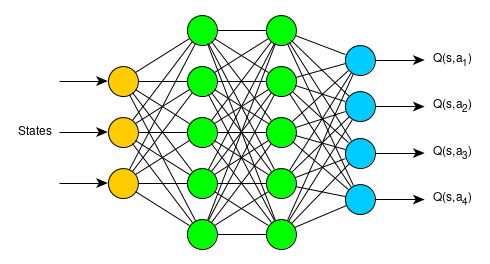
\includegraphics[width=0.9\columnwidth]{figures/q_network.png}
	\label{fig:q_network_illustration}
	\caption{Illustration of a neural network with $3$ state inputs and $4$ q-value outputs that can be mapped to actions.}
\end{figure}


The neural network is trained by a method called experience replay that is based on simulating the system and recording all states, rewards and actions taken in memory.
The simulation ends when it reaches a termination condition that is defined in the environment.
For the double pendulum case the termination condition is when the outer pendulum angle becomes larger than a defined maximum value.
One full simulation from start to termination is called an episode.
The stored experience is used to fit the neural network once there is enough experience stored in the memory.
\begin{equation}
	Exp \leftarrow \begin{pmatrix}s_t, & a_t, & r_t, & T_t, & s_{t+1}	\end{pmatrix}
\end{equation}
where $s_t$ is the state at time t, $a_t$ the action taken by the system at time t, $r_t$ the gained reward for the taken action, $T_t$ indicating whether the system has terminated and $s_{t+1}$ the next state in time.
The experience is used to map a target for the neural network training.
Targets are q-values for each action given a state.
Since the experience only holds data about the actual action that was taken for a given state the other q-values for the same state have to be estimated to complete the entire target vector.
There are several ways to estimate the unknown q-values for a given state.
Although the $NN_Q$ network can be used to predict the target values for the other actions it causes the targets to be non-stationary leading to the network chasing its own tail.
A separate neural network, $NN_{target}$, was used to avoid the non-stationary targets problem.
$NN_{target}$ has the same network architecture as $NN_Q$.
After a number of episodes the weights of $NN_Q$ are mapped to $NN_{target}$ to give better estimations of the unknown q-values.

\begin{algorithm}[H]
	\label{alg:deep_q_training}
	\caption{Deep Q-Learning}
	\begin{algorithmic}
		\For{episode $[0, \text{max episodes}]$ }
			\While{$t < t_{max}$ and $T_t$ is \False} \Comment{Simulate system}
				\State $q_{values} \gets NN_Q(s_t)$  % \Comment{Predict q-values for actions for current state}
				\State $a \gets argmax(q_{values})$ 	 \Comment{$a$ is index}
				\State $s_{t+1}, r_t, T_t \gets \text{Step}(ActionSpace[a])$ % \Comment{Simulate system one step}
				\State $Exp \gets \begin{pmatrix} s_t, & a_t, & r_t & T_t & s_{t+1} \end{pmatrix}$
				\State $\begin{pmatrix} \mathbf{s}, & \mathbf{a}, & \mathbf{r} & \mathbf{T} & \mathbf{s}_{t+1} \end{pmatrix}$ $\gets Exp$  \Comment{Exp minibatch}
				\State $y_m = \begin{cases} r_m \\ r_m + \gamma \max ( NN_{target}(\mathbf{s}_{t+1, m}) ) \end{cases}$
				\State $Targets_{m,j} \gets \begin{cases} y_m, & \text{if} \quad j = a  \\ NN_Q(\mathbf{s}_m)_j \end{cases}$
				\State $model.fit(\mathbf{s}, Targets)$
			\EndWhile
		\EndFor
	\end{algorithmic}
\end{algorithm}
The actual value $y_m$ replaces the corresponding predicted q-value from $NN_{target}(\mathbf{s}_m)$.
 Since we only have the reward for one action in a given state, we replace the targets for the untaken actions with a prediction from the Q-network. This will result in a loss of 0 for these untaken actions, thus not affecting the training.
 This way the network is trained only by the state-action pair that has been taken.

% \comment{Predict q-values for actions for current state}
% \comment{Pick largest q value and map it to the action}
% \comment{Simulate system one step}

% \begin{equation}
% 	\label{eqn:termination_condition}

% \end{equation}

%%%%%%%%%%%%%%%%%%%%%%%%%
%%%%%%%%%%%%%%%%%%%%%%%%%
% TODO
% * Termination condition - defined in the environment (simulation)
% * Bellman equation (5)
%%%%%%%%%%%%%%%%%%%%%%%%%
%%%%%%%%%%%%%%%%%%%%%%%%%




%Describe the control or learning system you have designed.
%Did you build anything? If so, what did you build, and using what production methods. If you built the hardware or were handed it, \emph{a photograph of your gadget is mandatory}. Make sure any figures are referenced from from the text---like this, see Figure~\ref{fig:gadget}---and that they all have a descriptive caption.
%\begin{figure}[b]
%	\centering
%	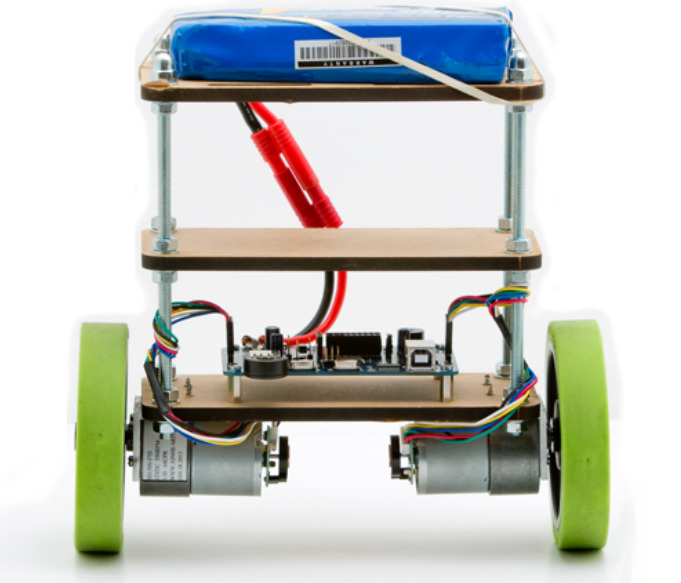
\includegraphics[width=0.7\columnwidth]{balanduino}
%	\caption{Example picture of the Balanduino robot. Place all figures at the top \texttt{[t]} (default) or bottom \texttt{[b]} (only if needed).}
%	\label{fig:gadget} % Should be placed after the caption!
%\end{figure}
%
%\subsection{Some Dummy Text}
%\kant[3]

\section{Implementation}
The project was implemented in \texttt{Python}.
A separate class was created for each component \texttt{Agent}, \texttt{Environment}, \texttt{Simulator} and \texttt{Controller}.
The goal of the project is to produce a \texttt{Controller} object that can control the \texttt{Simulator}.
\texttt{Environment} class contains the problem specifics such as \texttt{reward} and \texttt{termination} functions, and links the \texttt{Agent} with the \texttt{Simulator} containing the physical model dynamics.
\texttt{Agent} contains the learning algorithm that trains and produces the \texttt{Controller}.
The \texttt{Controller} is a simple object that produces the force to apply given the current state of the system.
\begin{equation}
	C := \mathbb{R}^M \to \mathbb{R}
\end{equation}

All components are independent of each other making the structure modular.
By using this structure it is easy to change for example the learning algorithm without having to modify anything else.

\subsection{Simulator}
The \texttt{Simulator} is responsible for the physical dynamics of the problem and for simulating the problem for given external inputs and time.
Equations are on the form of RHS-equations and are solved using \texttt{odeint} function in \texttt{Scipy.integrate} package.

\subsection{Environment}
The reward function and termination condition is implemented in the \texttt{Environment} class.
It acts as a connector between the \texttt{Agent} and the \texttt{Simulator}.
This way when the reward or the termination needs to be changed it can be done without altering the learning algorithm (\texttt{Agent}) or the physical model \texttt{Simulator}.

% Reward function : only look at the angle, not the velocity
% 					don't want the algorithm to sacrifies angle for velocity ... something like that.

% Here you describe how you implemented your learning or control design.

\begin{figure}[H]
	\centering
	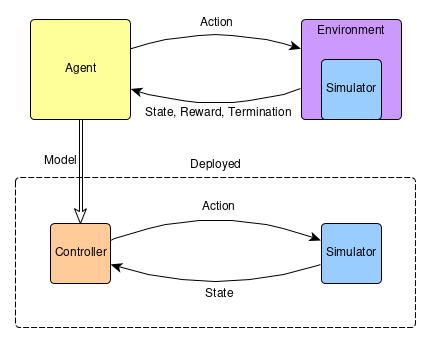
\includegraphics[width=0.9\columnwidth]{figures/CodeStructure.png}
	\label{fig:code_architecture}
	\caption{Code architecture.}
\end{figure}

\subsection{Evaluation}
\texttt{Controller} is evaluated after a set of episodes in order to keep track of the controller performance.
Performance is measured by averaging the total reward for $N_{eval}$ simulations of the dynamic system controlled by the \texttt{Controller}.
\begin{equation}
	\label{eqn:evaluation_equation}
	\frac{1}{N_{eval}} \sum_i^{N_{eval}} \sum_j^{M_i} R(s_j)
\end{equation}
Notice that the number of simulation steps $M_i$ for each simulation varies as a simulation may reach a termination condition sooner or later than another simulation.
% $\mathbf{R}_i$ is the total reward for the $i$th simulation of the controlled dynamic system.
A satisfactory evaluation value can be used as a termination condition for the training to avoid overtraining.
This mechanism has not yet been implemented.
The training will continue until the max iterations have been reached.



\section{Results}
A simpler problem was used to confirm the implementation.
The simpler problem being to balance a single inverted pendulum on a cart.
The implementation architecture was used to simply replace the environment with one suitable for the single pendulum problem.
% Once satisfied with the algorithm implementation the double pendulum problem was run.

\subsection{Balancing Single Inverted Pendulum}
The single pendulum problem is non-chaotic.
Equations from \cite{Correct_Equations} were used to model the problem.
System was terminated when the pendulum angle was grater than $\pm 10$ degrees.
Equation \eqref{eqn:reward_single_pendulum} states the reward function.
\begin{equation}
    \label{eqn:reward_single_pendulum}
    R(s) = (\theta_{max} - |\theta|)/ \theta_{max}
\end{equation}
where $\theta_{max} = 10$ degrees.

Table \ref{table:params_q_network} shows the neural network setup for the single pendulum problem.
\begin{table}[H]
    \centering
    \begin{tabular}{|
    >{\columncolor[HTML]{CBCEFB}}c |c|c|}
    \hline
    \cellcolor[HTML]{9AFF99}\textbf{Layer} & \cellcolor[HTML]{9AFF99}\textbf{Number of Neurons} & \cellcolor[HTML]{9AFF99}\textbf{Activation} \\ \hline
    \textbf{Input}                         & 4                                                  & -                                           \\ \hline
    \textbf{Hidden 1}                      & 20                                                 & ReLU                                        \\ \hline
    \textbf{Hidden 2}                      & 40                                                 & ReLU                                        \\ \hline
    \textbf{Output}                        & 4                                                  & Linear                                      \\ \hline
    \end{tabular}
    \caption{Network parameters for the Q-network}
    \label{table:params_q_network}
\end{table}

Table \ref{table:params_pendulum} shows the training parameters for the single pendulum problem.

\begin{table}[H]
    \centering
    \begin{tabular}{|
    >{\columncolor[HTML]{FFCE93}}c |
    >{\columncolor[HTML]{ECF4FF}}c |}
    \hline
    \textbf{Max Angle}     & 10             \\ \hline
    \textbf{Step Size}     & 0.02           \\ \hline
    \textbf{Action Space}  & {[}-10,0,10{]} \\ \hline
    \textbf{Learning Rate} & 0.1            \\ \hline
    \textbf{Memory}        & 2000           \\ \hline
    \textbf{Batch Size}    & 32             \\ \hline
    \textbf{Discount}      & 0.9            \\ \hline
    \end{tabular}
    \caption{Parameters for the Deep Q-learning algorithm on the single pendulum problem. }
    \label{table:params_pendulum}
\end{table}

Figure \ref{fig:single_pendulum_eval} shows the agent performance over episodes.
The agent starts to learn how to move the cart to increase the score after a few episodes.
Eventually the reward gain stops increasing.
The system was simulated with the maximum $200$ steps for each episode, capping the max possible reward to $200$.
However, $200$ is only possible if the initial condition starts in the equilibrium point.
The initial condition for each episode is randomized preventing the system from reaching $200$ score in the evaluation.

\begin{figure}[H]
	\centering
	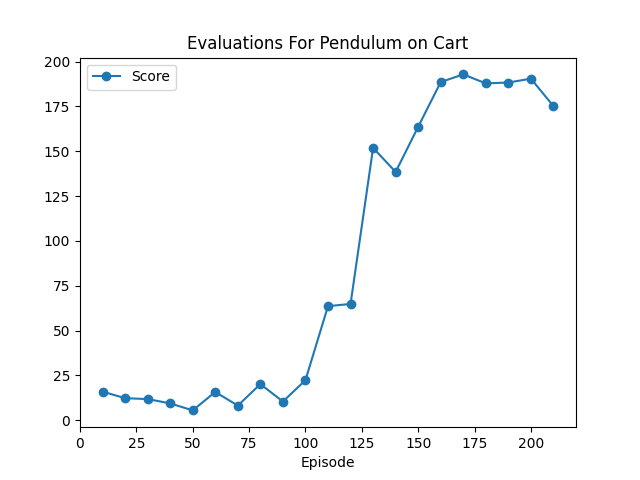
\includegraphics[width=0.9\columnwidth]{figures/SinglePendulum_eval.png}
	\label{fig:single_pendulum_eval}
	\caption{Evaluated controller score for every $10$ episodes. The evaluation is measured as the average score of $10$ full controlled simulations. Maximum number of steps for each evaluation iteration was $200$, capping the maximum possible reward to $200$.}
\end{figure}

Figure \ref{fig:single_pendulum_angle} shows the pendulum angle over time for training episode $170$.
It seems as if the system is learning which direction to push the cart to get the pendulum closer to the equilibrium point.
The curve from time $0.5$ to $2.5$ also indicates that the system is starting to understand that it needs to slow down the pendulum before reaching equilibrium to prevent overshooting.
However, later on it seems to start oscillating around the equilibrium.

\begin{figure}[H]
	\centering
	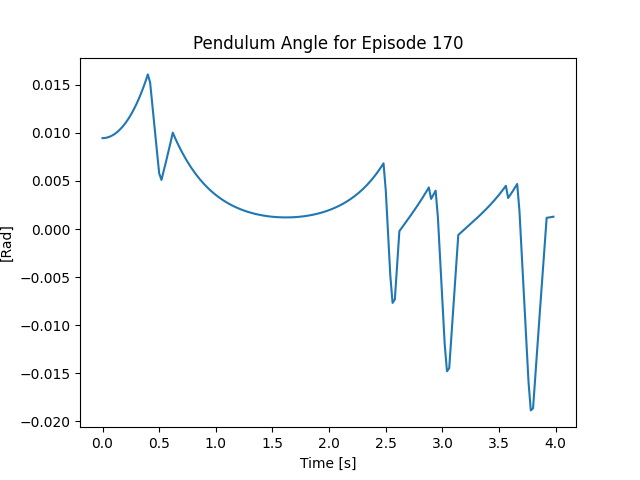
\includegraphics[width=0.9\columnwidth]{figures/Pendulum_angle.png}
	\label{fig:single_pendulum_angle}
	\caption{Pendulum angle over time for training episode $170$.}
\end{figure}

The trained controller was used to control the single pendulum for initial conditions outside the trained domain, and the controller managed to bring back the pendulum to the known domain and balance it.
This can be seen in figure \ref{fig:single_pendulum_outside_training_domain}.
Results indicate that the network has managed to generalize the problem.
This would not be possible with a regular Q-table approach since the agent has never seen the states outside the training domain and would end up performing random actions.

\begin{figure}[H]
	\centering
	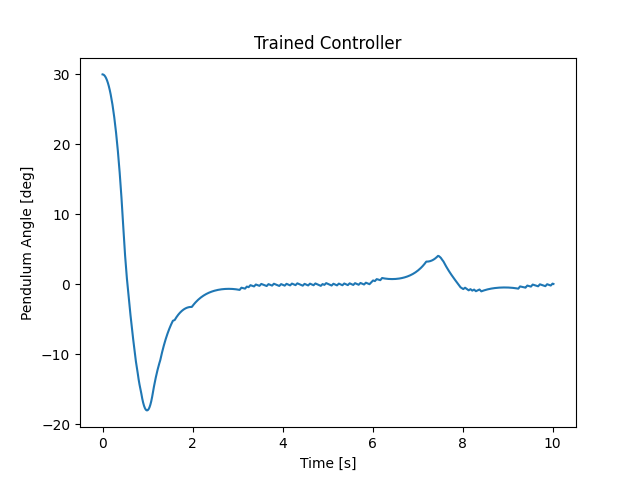
\includegraphics[width=0.9\columnwidth]{figures/Pendulum_angle_30.png}
	\caption{Changes in pendulum angle $\theta$ over time for controlled simulation of single pendulum on cart problem. The initial condition was $\theta = 30$ degrees.}
	\label{fig:single_pendulum_outside_training_domain}
\end{figure}


% If you need to use tables, Table~\ref{tab:extable} shows an example of how they can be typeset. For further details, see \cite{tablelatexwiki}.

\subsection{Balancing Double Inverted Pendulum}
Results are currently not sufficient.
Various experiments are being conducted with different hyper parameters such as network sizes, different action spaces, learning rates etc.
A problem with tuning hyper parameters is the long feedback loop coming from long training times.

The termination condition is given by equation \eqref{eqn:termination_double_pendulum}.
\begin{equation}
	\label{eqn:termination_double_pendulum}
	y_{outer} < y_{min}
\end{equation}
$y_{outer}$ is the height of the outer pendulum bob and $y_{min}$ the minimum height allowed for the bob.
Reward is given by equation \eqref{eqn:reward_double_pendulum}
\begin{equation}
	\label{eqn:reward_double_pendulum}
	R(s) = (\theta_{max} - |\theta_{outer}|) / \theta_{max}
\end{equation}
with $\theta_{max} = 5$ degrees.

\begin{figure}[H]
	\centering
	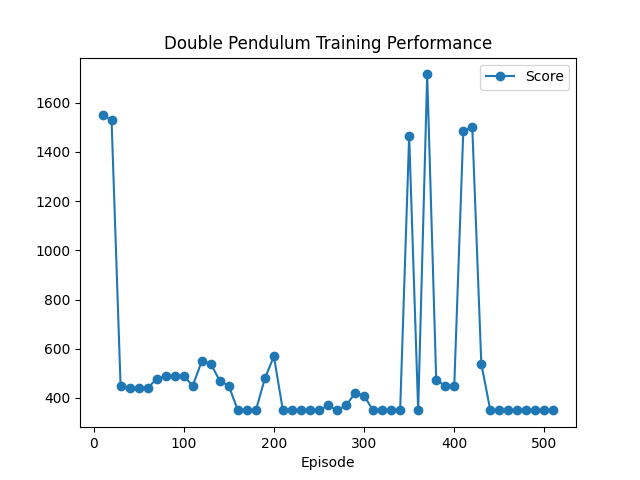
\includegraphics[width=0.9\columnwidth]{figures/double_pendulum_eval.png}
	\caption{Current results for training the controller.}
	\label{fig:double_pendulum_score}
\end{figure}
Although this method works for the single pendulum case, since the double pendulum is a highly chaotic system, the algorithm is having a difficult time training the controller as seen in Figure \ref{fig:double_pendulum_score}.
We believe that the reason for this could be that the hyper parameters are not optimal or we are not giving the algorithm enough time to train even though the training takes several hours.
\section{Discussion}
While training a controller for the double pendulum problem, we saw that for some cases after the average score increases for a while, it suddenly starts to decrease and can remain there untill the training ends.
We think that this may be a result of the hyper parameter choices such as network architecture.
We believe that this may be an effect such as overtraining or that the network is too simple.
We are trying different combinations in order to understand this behavior.
Also, as seen in Figure \ref{fig:double_pendulum_score}, we are getting sudden spikes during training.
We are also currently trying to understand this phenomenon.
\section{Project Plan}
The initial project plan was followed quite well.
However, the time to tune hyper parameters for the double pendulum problem were underestimated.
Work on that part still remains.
One problem for tuning the hyper parameters is that the feedback loop for a single change is long.
It takes a long time to train the controller for the double pendulum and therefore a long time before hyper parameters can be adjusted.
Figure \ref{fig:gantt_chart} shows the updated Gantt chart.
The green colored blocks are completed steps.
Blue blocks are work in progress.
\begin{figure}[H]
   \centering
   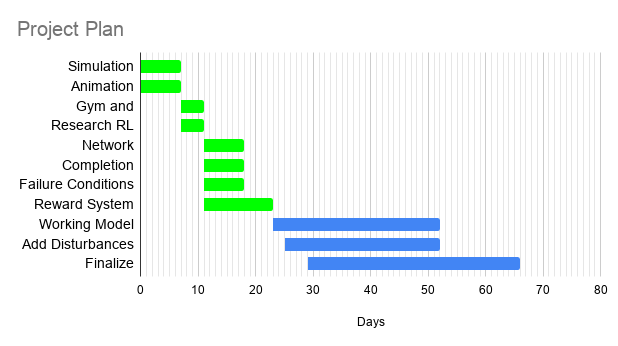
\includegraphics[width=0.9\columnwidth]{figures/Revised_Project_plan.png}
   \caption{Revised Gantt chart.}
   \label{fig:gantt_chart}
\end{figure}
% Prints cited references
\printbibliography
\end{document}
